\part{GELİŞTİRİLEN YÖNTEM}
\thispagestyle{empty}
\newpage
\section{YENİLENEBİLİR ENERJİ SİSTEMLERİ İÇİN\\DAĞITIK ALGILAYICI AĞ MİMARİLERİ: DPÜ MODELİ}

 Başlık \ref{motivasyon} bize haberleşme sistemlerinin enerji sistemlerinde nasıl kullanıldığı hakkında geçmişte yapılmış olan araştırmaları özetlemiştir. \gls{dpu}'de tüm enerji ihtiyacını yenilenebilir kaynaklardan karşılaması için bir çalışma yapılması durumu düşünüldüğünde, bu tezin \ref{motivasyon} ve \ref{onem} kısımlarında bahsi geçen konular dikkate alınması gerekmektedir. Çünkü enerji sisteminde karşılaşılan problemlerin sonuçları, ilgili sistemlerin sahibine maddi açıdan yüklü maliyetler oluşturabilir. İlgili sorunların önüne geçilmesi için \gls{dpu}’ye ait tüm eğitim lokasyonlarının aktif ve sürekli bir şekilde merkezi bir yapıdan enerji üretiminin izlenmesi, kontrolünün sağlanması ve olası problemleri önceden tahmin edebilmesi için üretim sistemlerine ait tüm cihazların durum ve faaliyetleri hakkındaki veri trafiğini incelemesi gerekir. \gls{dpu}’ye ait lokasyonlarda güneş veya rüzgar enerji santrallerinin kurulduğu varsayılmıştır. Tezin giriş kısmında belirtilen rüzgar ve güneş enerji sistemlerinin dışındaki diğer yenilenebilir enerji sistemleri bu yüksek lisans tezinde incelenmemiştir.

Güneş enerjisi ve rüzgar enerji santrallerinin kapasite faktörünün düşük olma-sının temel nedeni genellikle enerji kaynağının her zaman kullanılabilir olmaması durumundan kaynaklıdır. Tesis elektrik üretebiliyor olabilir, ancak "yakıtı" (rüzgar, güneş ışığı) mevcut olmayabilir. Bununla birlikte, güneş, rüzgar santralleri yüksek kullanılabi-lirlik faktörlerine sahiptir, bu nedenle mevcut yakıtları olduğunda neredeyse her zaman elektrik üretebilirler. Genelleme yapıldığında Rüzgar tarlalarında kapasite faktörü \%20--40 arasında olurken, güneş panellerinde \%15--30 arasında olmaktadır \cite{hussain2014multilayer}. Türkiye Cumhuriyeti Enerji ve Tabii Kaynaklar Bakanlığı’nın yayınlamış olduğu enerji haritalarından Kütahya’ya ait rüzgar ve güneş enerji kapasitelerini Şekil \ref{fig:figure7}--\ref{fig:figure8} üzerinde gösterilmiştir \cite{gepa}\cite{repa}. İlgili resimlerle gösterilmiş olan kapasite faktörleri değerlendirilmiştir. Buna göre üniversite yerleşkelerine kurulması muhtemel enerji sistemleri Tablo \ref{tab:tabb1}'de gösterilmiştir.

\begin{figure}[htbp]
\centerline{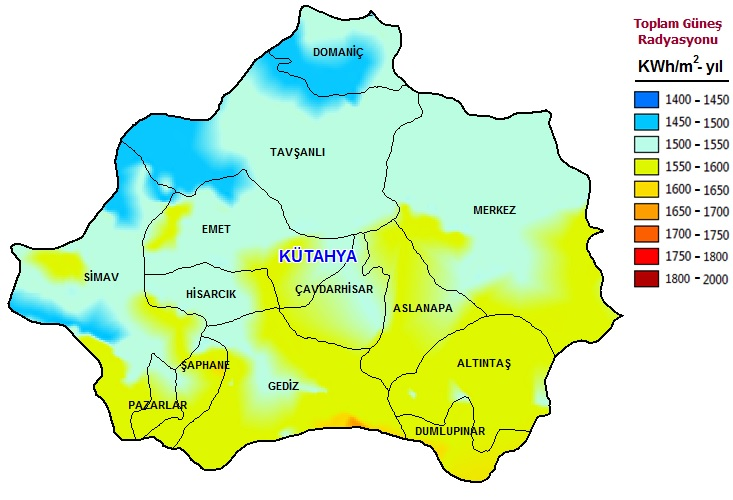
\includegraphics[width=\columnwidth]{Resim/Sekil3-1.jpg}}
\caption{Kütahya bölgesi güneş enerjisi atlası  (\protect\citeA{gepa}) }
\label{fig:figure7}
\end{figure}

%\section{Enerji Üretilecek Yöntemin Seçimi}


\section{HABERLEŞME AĞI TASARIM KONSEPTİ}

İletişim, bir organizasyonun başarısındaki en önemli faktörlerden biridir. Bir kurum, ancak haberleşme ağ altyapısı güçlüyse, iş akış ve takip süreçleri kolaylaşır sürdürü-lebilir bir yapıda olur. Bu nedenle organizasyonlar ve kurumlar arasında kapsamlı bir şekilde haberleşme yapıları kurulmuştur. Ağ hizmetleri, ağın uygulanmasını, yönetimini, bakımını ve izlenmesini gibi görevleri üstlene bir yapıdır. Buna göre ağ hizmetlerinin sorunsuz bir şekilde sağlanması için hizmette kullanılan bileşenler aşağıdaki başlıklarda incelenmiştir.



\begin{figure}[htbp]
\centerline{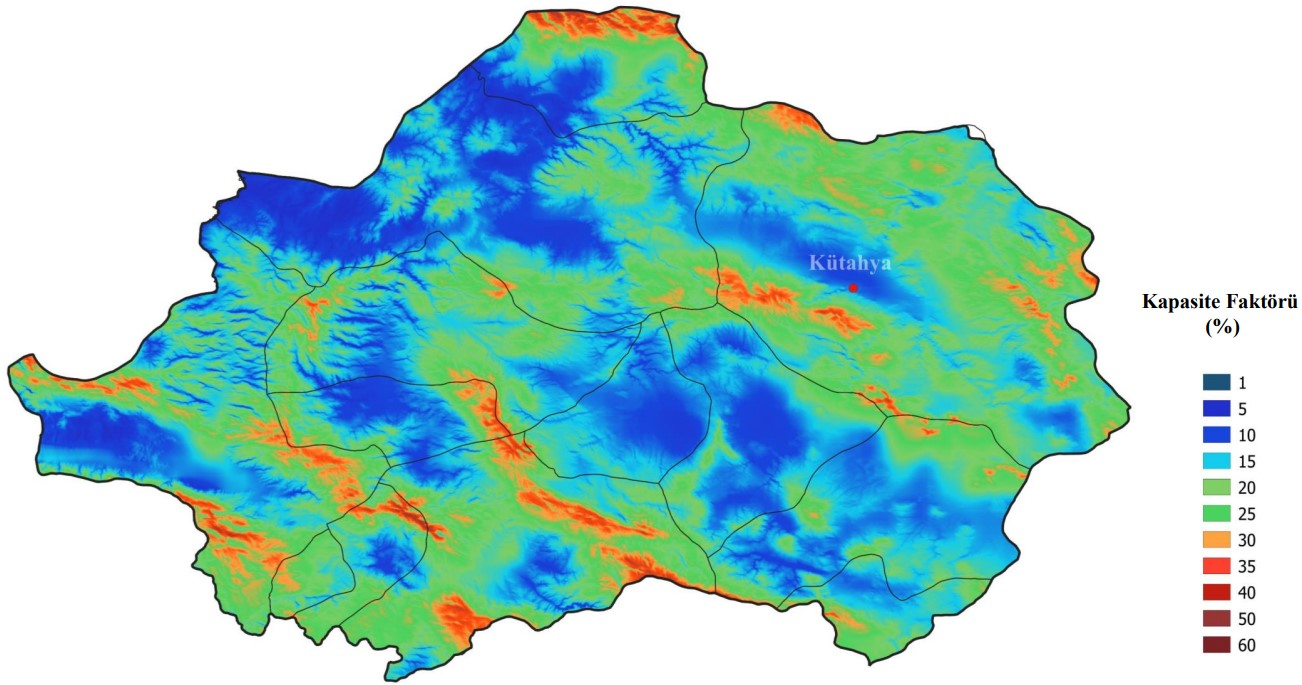
\includegraphics[width=\columnwidth]{Resim/Sekil3-2.jpg}}
\caption{Kütahya bölgesi rüzgar enerjisi atlası  (\protect\citeA{repa}) }
\label{fig:figure8}
\end{figure}

\begin{table}[htbp]
\centering
\caption{\gls{dpu}'nün yerleşkelerinde kurulacak olan enerji sistemlerinin tablosu}
\label{tab:tabb1}
\begin{tabular}{clccc}
\hline
No & \multicolumn{1}{c}{Yerleşke İsmi} & \multicolumn{1}{c}{Enerji Sistemi} & Enlem & Boylam \\ \hline
1  & ALTINTAŞ \gls{myo}    & \gls{ges}  & 39.07502 & 30.13237 \\
\hline
2  & ÇAVDARHİSAR \gls{myo} & \gls{ges}  & 39.18129 & 29.60534 \\
\hline
3  & DOMANİÇ \gls{myo}     & \gls{res} & 39.80160 & 29.60133 \\
\hline
4  & EMET \gls{myo}        & \gls{res} & 39.33699 & 29.26823 \\
\hline
5  & GEDİZ \gls{myo}       & \gls{ges}  & 39.00807 & 29.40444 \\
\hline
6  & GERMİYAN \gls{myo}    & \gls{res} & 39.39076 & 30.03973 \\
\hline
7  & HİSARCIK \gls{myo}    & \gls{res} & 39.25412 & 29.22920 \\
\hline
8  & PAZARLAR \gls{myo}    & \gls{ges}  & 28.99846 & 29.12381 \\
\hline
9  & ŞAPHANE \gls{myo}     & \gls{ges}  & 39.02577 & 29.22203 \\
\hline
10 & SİMAV \gls{myo}       & \gls{res} & 39.11189 & 29.01717 \\
\hline
11 & TAVŞANLI \gls{myo}    & \gls{res} & 39.56802 & 29.45904\\
\hline

\end{tabular}
\end{table}
\subsection{Ağ Bileşenleri}

Tezin giriş kısmında bahsedildiği üzere iletişim olanakları arasında telefon hatları, koaksiyel kablolar, mikrodalga bağlantıları, uydu kanalları ve optik fiberler bulunmaktadır. Bu fiziksel ortamların her biri, iletişimi sağlama yeteneği açısından farklı özelliklere sahiptir. Ağ tasarımının kriterleri genelde maliyet, kapasite ve güvenilirlik olarak 3 kısımdan oluştuğunu düşünebiliriz. Aylık kiralama maliyeti, kurulum maliyeti, birim trafik başına maliyet ve bakım onarım maliyeti olarak olarak dört kısımda toplanır. Ağ tasarımındaki metodolojiye göre bu maliyetler hesaplanır. Kapasite tarifi genelde veri haberleşmesi olduğundan bit/s olarak saniyede taşınan veri miktarı olarak tanımlanır. Haberleşme uygulamalarında toplam kapasitenin tamamında haberleşme mesajları bulunmamaktadır. Sayısal haberleşmede kullanılan bir takım haberleşme protokolleri verinin önüne ve sonuna protokol mimarisini anlatan veri paketleri üretmektedir. Bu yüzden kullanılabilir kapasite ile toplam kapasite arasında veri boyutu farkı oluşmaktadır. Güven Oranı hesabı bir kanalın faal ve gayri faal olduğu zamanın oranı olarak tanımlanabilir. Bu tanıma göre gayri faal olma aralığı (GFOA) ile gayri faal süresi (GFS) bileşenleriyle Denklem \eqref{eq1}'de hesaplanır. 

\begin{equation}
\text{Güven Oranı} = 1 - (\text{ GFS / GFOA } ) \label{eq1}
\end{equation}


Haberleşme ağlarının oluşumunda kullanılan cihazlara genelde düğüm olarak isim verilmektedir. Ağ düğümlerini aşağıdaki gibi sınıflara ayırabiliriz \cite{parziale_2006}.




\subsubsection{Hub(Cihaz Aktarıcı)}

Hub'lar, birden çok ağ aygıtını birbirine bağlar. Hub aynı zamanda bağlantı kabloları üzerinden uzun mesafeler kat ettikten sonra bozulan sinyalleri güçlendirdiği için bir tekrarlayıcı görevi görür. Hub, yerel ağ bileşenlerini aynı protokollerle bağladığı için ağ bağlantı cihazları ailesinde en basit olanıdır.

Verilerin biçimlendirilmesine hazırlanmak üzere yapılandırılması koşuluyla hem sayısal hem de analog verilerle kullanılabilir. Örneğin, gelen veri sayısal formatta ise, hub bunu paketler halinde iletmesi gerekir; ancak gelen veri analog ise, hub bunu sinyal biçiminde iletir.

Hub'lar, paket filtreleme veya adresleme işlevleri gerçekleştirmez; sadece bağlı tüm cihazlara veri paketleri gönderirler \cite{parziale_2006}.




\subsubsection{Switch (Ağ Anahtarı)}

Genellikle Hub’dan daha akıllı cihazlar olarak sınıflandırılır. Anahtar, ağdaki düğümler hakkında sınırlı yönlendirme bilgilerini korur ve hub’lar veya yönlendiriciler gibi sistemlere bağlantı izni verir. Yerel ağ tasarımında genelde anahtar kullanılır.

Anahtarların sahip olduğu sanal ağ yapılandırma tekniği sayesinde hublara göre çok tercih edilir. Anahtarların ağ güvenliği sanal ağ yapılandırma tekniğinden dolayı daha güvenlidir \cite{parziale_2006}.



\subsubsection{Yönlendirici (Router)}

Farklı ağ topolojilerinin kullanılmış olduğu yapılar arasında çizilen patikadaki veri trafiğini sağlayan cihazlara yönlendirici tanımı yapılmaktadır. Yönlendiriciler akıllı cihazlardır ve bağlı oldukları ağlar hakkında bilgi depolarlar. Yönlendiriciler, geniş alan ağlarında kapsayacak şekilde bir tasarıma geçmektedir. birden çok yerel ağı birbiriyle haberleştirmeyi sağlar. Haberleştirme sırasında tanımlanan veri trafiklerine göre rotalar oluşturur. Bu tür yönlendiricilere sınır yönlendirici ismi de verilmektedir  \cite{parziale_2006}.

\subsubsection{Köprü (Bridge)}


Köprüler, yalnızca fiziksel veri bağlantı katmanlarında çalışmaktadır. Köprüler, iki fiziksel ağın arasında kurulur ve ikisi arasındaki veri akışını yönetir. Hub donanımına benzer bir yapısı vardır. Fakat veri paketlerini iletmeden önce hedef adresler için filtreleme özelliğini yapar. Köprüler işlevsellik açısından anahtarlardan daha az özelliğe sahiptirler. Maliyet açısından anahtarları kullanmak daha çok tercih edilmektedir \cite{parziale_2006}.


\subsubsection{Algılayıcı Düğümleri (Sensor Node)}\label{algilayicidugum}

Algılayıcı düğümleri, bu tezde kullanılan temel donanımdır. Çünkü enerji sistemlerinde üretilen bütün veriler bu algılayıcı düğümlerinde oluşturulacaktır. Çevresel durumları ölçerek haberleşme altyapısına uyacak veri şekillendirmesini yapar ve veri aktarım standartlarına göre veriyi hazırlayıp çalıştığı yerel ağına bağlı olan sunucuya ölçmüş olduğu algılayıcı verilerini gönderirler. Algılayıcıların göndermiş olduğu veri detayları 4. bölümde verilecektir \cite{parziale_2006}.

\begin{figure}[htbp]
\centerline{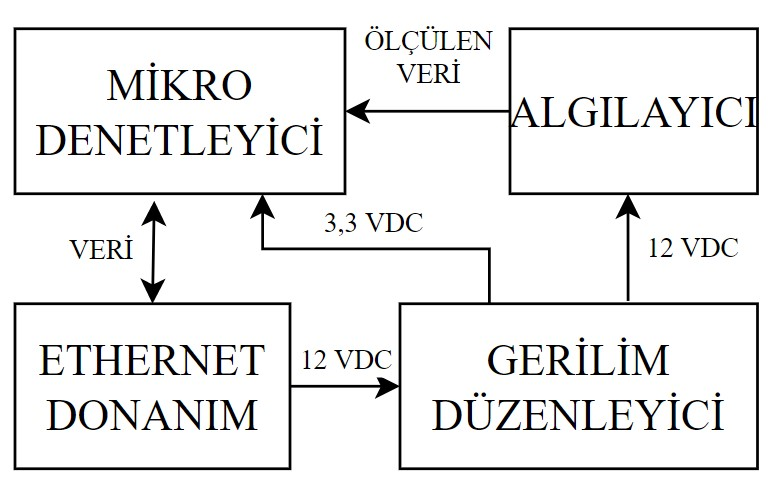
\includegraphics[width=10cm]{Resim/sekil3-3.jpg}}
\caption{Ethernet tipi algılayıcı düğümü gösterimi}
\label{fig:figure9}
\end{figure}

Şekil ~\ref{fig:figure9}'teki resme bakıldığında ethernet tabanlı algılayıcı düğümünün blok diyagramı gösterilmiştir. Haberleşme trafiği ve cihazın ihtiyaç DC gerilim ethernet kablosuyla aktarılmaktadır.


\begin{figure}[htbp]
\centerline{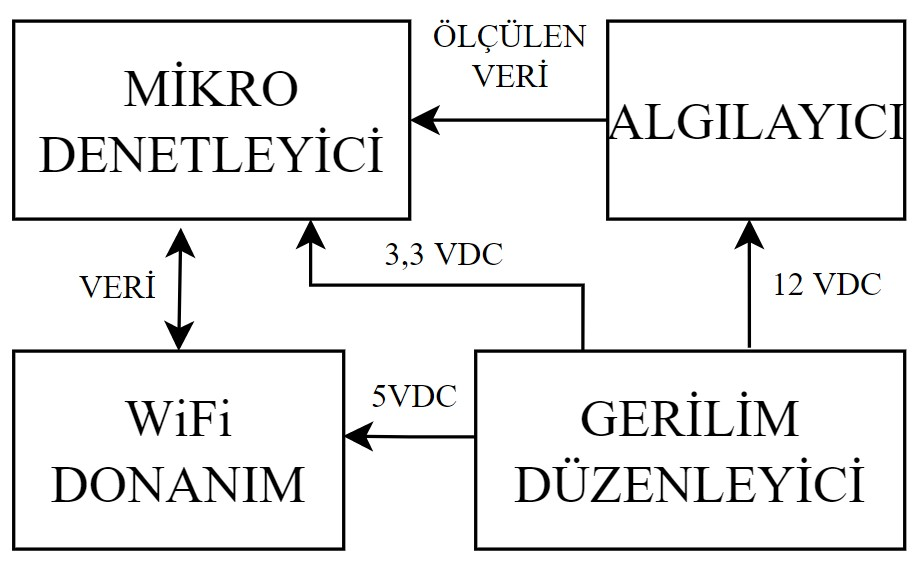
\includegraphics[width=10cm]{Resim/sekil3-4.jpg}}
\caption{Kablosuz tipi algılayıcı düğümü gösterimi}
\label{fig:figure10}
\end{figure}

Şekil ~\ref{fig:figure10}'teki resme aynı algılayıcı düğümünün kablosuz haberleşme modelinin blok diyagramı paylaşılmıştır.

\subsection{Haberleşme Ağ Sınıfları}


\subsubsection{Kişisel Alan Ağı (PAN)}
Cihazlar arası çok düşük mesafede haberleşme imkanı sağlayan ağlara kişisel alan ağı denir \cite{tanenbaum2002computer}.

\begin{figure}[htbp]
\centerline{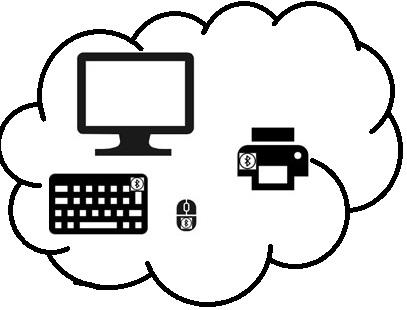
\includegraphics[width=8cm]{Resim/Sekil3-5.jpg}}
\caption{Bilgisayara bağlı olan bluetooth bağlantılı cihazların oluşturduğu \gls{pan} ağı gösterilmiştir.}
\label{fig:figure11}
\end{figure}

\subsubsection{\gls{lan}}
\gls{lan}'lar, kişisel bilgisayarın veya elektronik cihazların bilgi alışverişinde bulunmalarına izin vermek için oluşturulan ağa denir. Günümüzde özellikle kablosuz yerel ağlar kolayca gözlemlenebilir. Kafeteryadaki kablosuz ağlara kişisel bilgisayarları, telefonları veya tablet bilgisayarlarıyla bağlanan kişiler, aslında internet hizmetinden faydalanabilmek için yerel ağa bağlanmış olurlar. Kablosuz ağa dahil olabilmek için gereken anten modülüne sahip ağ adaptörünün olmasıdır. Genelde bilgisayarlar ve elektronik cihazlar kablosuz bir şekilde haberleşme yapabilmek için Erişim Noktası (Access Point), kablosuz yönlendirici veya baz istasyonlarına bağlanırlar \cite{tanenbaum2002computer}.

\begin{figure}[htbp]
\centerline{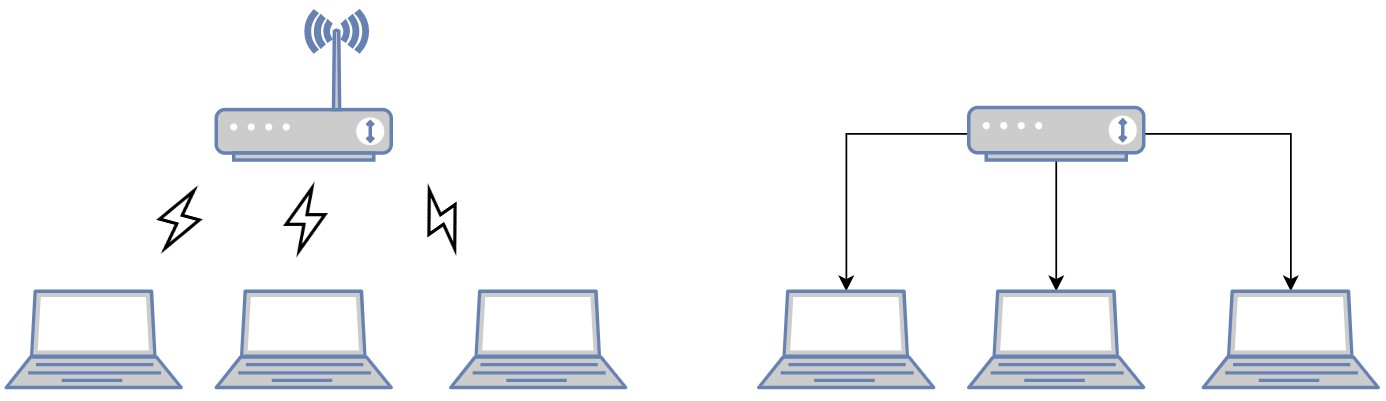
\includegraphics[width=\columnwidth]{Resim/Sekil3-6.jpg}}
\caption{\gls{lan} gösterimi.}
\label{fig:figure12}
\end{figure}

\subsubsection{MEtropolitan Alan Ağı (\gls{man})}

\gls{man}'ın en bilinen örnekleri kablolu televizyonlardır. İletişim firmaları tüm şehirleri kablolamak için yerel yönetimlerle sözleşme üzerinden televizyon yayını için altyapı çalışmalarında bulunmuştur. Televizyonun yayın trafiği için tasarlanan kabloları, internetin geniş bir kitleyi kendine çekmeye başladığı zaman, kablolu TV şebekesi operatörleri, sistemde yapılacak bazı değişikliklerle, yayın spektrumunun kullanılmayan kısımlarında iki yönlü internet hizmeti sağlayabileceklerini buldular. Bu noktada, kablolu TV sistemi, televizyonu bir \gls{man} dağıtmanın basit bir yolundan dönüşmeye başladı. İlk yaklaşıma göre, bir \gls{man} Şekil \ref{fig:figure13}'de gösterilen topoloji gibidir. Bu şekilde, hem televizyon sinyalleri hem de internet daha sonra insanların evlerine dağıtılmak üzere merkezi kablolu modem sonlandırma sistemine evrilmiştir. \cite{tanenbaum2002computer}.


\begin{figure}[htbp]
\centerline{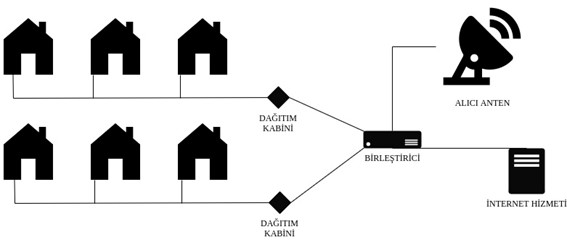
\includegraphics[width=\columnwidth]{Resim/Sekil3-7.jpg}}
\caption{\gls{man} örnek gösterimi.}
\label{fig:figure13}
\end{figure}

\subsubsection{\gls{wan}}

\gls{wan}, geniş bir coğrafi alanı, genellikle bir ülkeyi, bir kıtayı ve hatta birden çok kıtayı kapsar. Geniş bir ağ, bir kurumsal geniş alan ağı durumunda olduğu gibi özel bir kuruluşa hizmet edebilir veya bir transit ağ durumunda olduğu gibi ticari bir hizmet sunumu olabilir.
İzmir, Ankara, Sinop şehirlerinde şubeleri olan bir şirket örneğine ait bir \gls{wan} sistemi aşağıdaki şekilde gösterilmiştir. Bu şubelerin her biri, kullanıcı programlarını çalıştırmaya yönelik bilgisayarlar içerir. Şekilde gösterilen her şubeye ait makineler ana bilgisayar (host) olarak adlandırılır. Bu ana bilgisayarları birbirine bağlayan ağın geri kalanına iletişim alt ağı(subnet) denir. Telefon sisteminin sözcükleri konuşmacıdan dinleyiciye taşıması gibi, alt ağ da mesajları ana bilgisayardan ana bilgisayara taşır.
Çoğu geniş alan ağında, alt ağ iki farklı bileşenden oluşur: iletim hatları ve anahtarlama elemanları. İletim hatları sayesinde veriler makineler arasında taşınır. Bakır tel, koaksiyel kablo, optik fiber veya radyo teknolojileri iletim hatlarına örnek olarak gösterilir. Aşağıdaki resimde geniş alan ağı gösterilmiştir \cite{tanenbaum2002computer}.

\begin{figure}[htbp]
\centerline{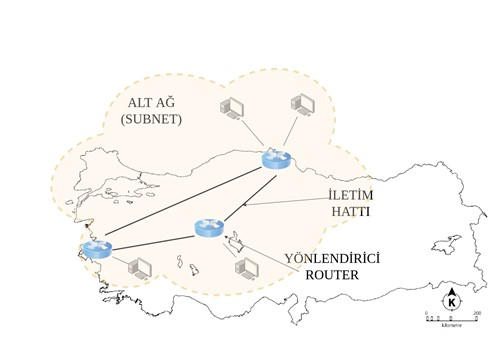
\includegraphics[width=12cm]{Resim/Sekil3-8.jpg}}
\caption{\gls{wan} örnek gösterimi.}
\label{fig:figure14}
\end{figure}


\subsection{Ağ Tasarım Yazılımı}

Ağ tasarım programlarının dünyada önemli bir rolü vardır. Çünkü haberleşme ağlarının sahada kurulumundan önce maliyet analizi ve performansının hesaplanması için çok bileşen bulunmaktadır. Piyasadaki ağ tasarım programları sayesinde, saha uygulaması yapılmadan maliyet hesabını ve uygulanabilirliğinin analizi mümkündür. \gls{opnet} yazılımı piyasada kullanılan en popüler ağ tasarım yazılımlarından birisidir. \gls{opnet} açık kaynaklı bir ürün değildir. Erişim ve kullanım için lisansa ihtiyaç bulunmaktadır. Özellikle ticari amaçlarla kullanılmasından kaynaklı olarak, kendi sitesinde ve haberleşme ağları tasarım dünyasında \gls{opnet} hakkında yazılmış çok sayıda kitap ve makale bulunmaktadır. \gls{opnet} yazılımın özellikleri;

•	Kolay bir grafik arayüzüne sahiptir.

•	Kullanıcılara zengin bir ağ modeli ve ağ tasarım kütüphanesi sunmaktadır.

•	Kullanıcı kolayca senaryo analizini yapabilmektedir.

•	Kurulumu diğer ağ tasarım programlarına göre daha kolaydır.

•	Grafik arayüzleri ile gerçek zamanlı bir simülasyon ortamı sağlar.

•	Ticari bir program olmasından kaynaklı güvenilir ve verimlidir.


\gls{opnet} çalışma prensibi olarak 4 bölümden oluşmaktadır. 

•	Model tasarımı

•	İstatistiklerin seçimi

•	Simülasyonun çalıştırılması

•	Elde edilen sonuçların görüntülenmesi ve analizi


Haberleşme ağlarında optimizasyon konulu bu yüksek lisans tezinde \gls{opnet} Akademik lisanslı yazılım kullanılarak simülasyon yapılmıştır. \cite{FITPUB8317}